\section{Interpretació de l'enunciat}
En aquest apartat s'expliquen les extensions i suposicions de l'enunciat original.

Tal i com es demana el programa està parametritzat segons la posició de la càmera,
el punt P que aquesta detecta i l'angle $\alpha$. A més existeixen altres paràmetres
com els punts on es troben les peces originalment i on es deixen al final, aquests
s'explicaran a l'apartat de punts.

Per altra banda s'ha introduït la possibilitat de fixar un nombre diferent de peces
a cada pila, per tant es poden tenir piles amb diferent número de peces. També
es te amb compte la possibilitat de tenir més d'una peça, o cap, d'algun tipus.

Tots aquests paràmetres es tornen a veure detallats en l'apartat d'explicació del
codi on s'expliquen les \emph{Macros pròpies}\ref{macprop}.

FIGURA AMB TOTS ELS PARÀMETRES

Finalment l'enunciat deixa oberta la possibilitat de que fer amb les peces de
tipus 4, en aquest punt s'ha optat per posar-les al pal 4 per aprofitar el codi ja escrit i
així seguir la coherència i estructura dels tipus de peça anteriors. El fet de
no optar per apilar-les en qualsevol punt de l'entorn es perquè en la paletització
ja s'ha demostrat coneixement de com apilar peces i tractar el tipus 4 de manera
diferent als anteriors minvava elegància al codi i l'execució.

\subsection{Moviment del robot}
En primer lloc el robot agafa les peces del les piles inicials.
Aquestes són co\lgem ocades a la zona de paletització. Un cop acabat amb la pinça
tombada agafa les peces començant per les que es troben més a l'esquerra
del braç robot, per co\lgem ocarles als pals. Així doncs al diagrama\ref{recpec}
veim quin seria l'ordre de recollida depenent dels diferents angles.

\begin{fibure}[H]
\begin{center}\label{fig:recpec}
 \includegraphics[width=0.8\textwidth]{ordreRotacions.png}
 % ordreRotacions.png: 1286x768 pixel, 150dpi, 21.77x13.00 cm, bb=0 0 617 369
\end{center}
  \caption{Ordre de recollida de les peces segons l'angle $\alpha$}
\end{figure}

Així doncs l'ordre de despaletització depen de l'angle i no del tipus de peça.
Com és pot veure a la figura existeixen 8 possibles casos que es veuen
reflectits en l'explicació del codi font corresponent \ref{casosrot}.

TODO dir mesures de seguretat en el moviment del braç